\documentclass[12pt]{article}

\usepackage{amsmath}    % need for subequations
\usepackage{graphicx}   % need for figures
\usepackage{verbatim}   % useful for program listings
\usepackage{color}      % use if color is used in text
\usepackage{subfigure}  % use for side-by-side figures
\usepackage{hyperref}   % use for hypertext links, including those to external documents and URLs
\usepackage{multicol}

\author{P.~Gusev}
\title{NDN-RTC app design and protocol specification (DRAFT v0.2)}

\begin{document}

\maketitle
\newpage

%************************************************
\section*{Abstract}
\tableofcontents

\newpage
\section{Overview}
\subsection{Participants and institutions}
\begin{multicols}{3}
\begin{itemize}
\item Alex Horn
\item Jeff Burke
\item Jeff Thompson
\item Peter Gusev
\item Lixia Zhang
\item Qiuhan Ding
\end{itemize}
\end{multicols}

\subsection{Motivation}
The video conferencing tool is one of those apps which is needed first of all for internal use and experimenting with real-time communication over NDN. As we are interested in increasing NDN popularity among non-research peers as well, we are trying to provide easy-to-setup NDN apps by employing web browser APIs. NDN-RTC is a JavaScript application which utilizes the WebRTC engine for media encoding/decoding and C++ NDN library for the transport layer.

\subsection{Description}
The main goal of NDN-RTC app is to provide real-time audiovisual communication between users and enable them to organize multiparty conferences. App should have simple intuitive user interface and should be easy-to-setup. 
The main functions provided by NDN-RTC app are represented by the Use-Case diagram on Figure \ref{fig:uc}. Main use cases of the app are the follows:
\begin{itemize}
\item \textbf{Discovery} 
\begin{itemize}
\item users should be able to discover other users of NDN-RTC app in order to start audio/video/text sessions with them;
\item users should be able to discover current ongoing multiparty conferencies.
\end{itemize}
\item \textbf{Join conference}
\begin{itemize}
\item users should be able to start new peer-to-peer or multiparty conference (audio-, video- or text-based);
\item users should be able to join existing conferences if they are allowed.
\end{itemize}
\item \textbf{Leave conference}
\begin{itemize}
\item users should be able to stop the conference they have initiated previously; 
\item users should be able to leave the conference they have joined previously.
\end{itemize}
\end{itemize} 

\begin{figure}[Hb!]
\centering
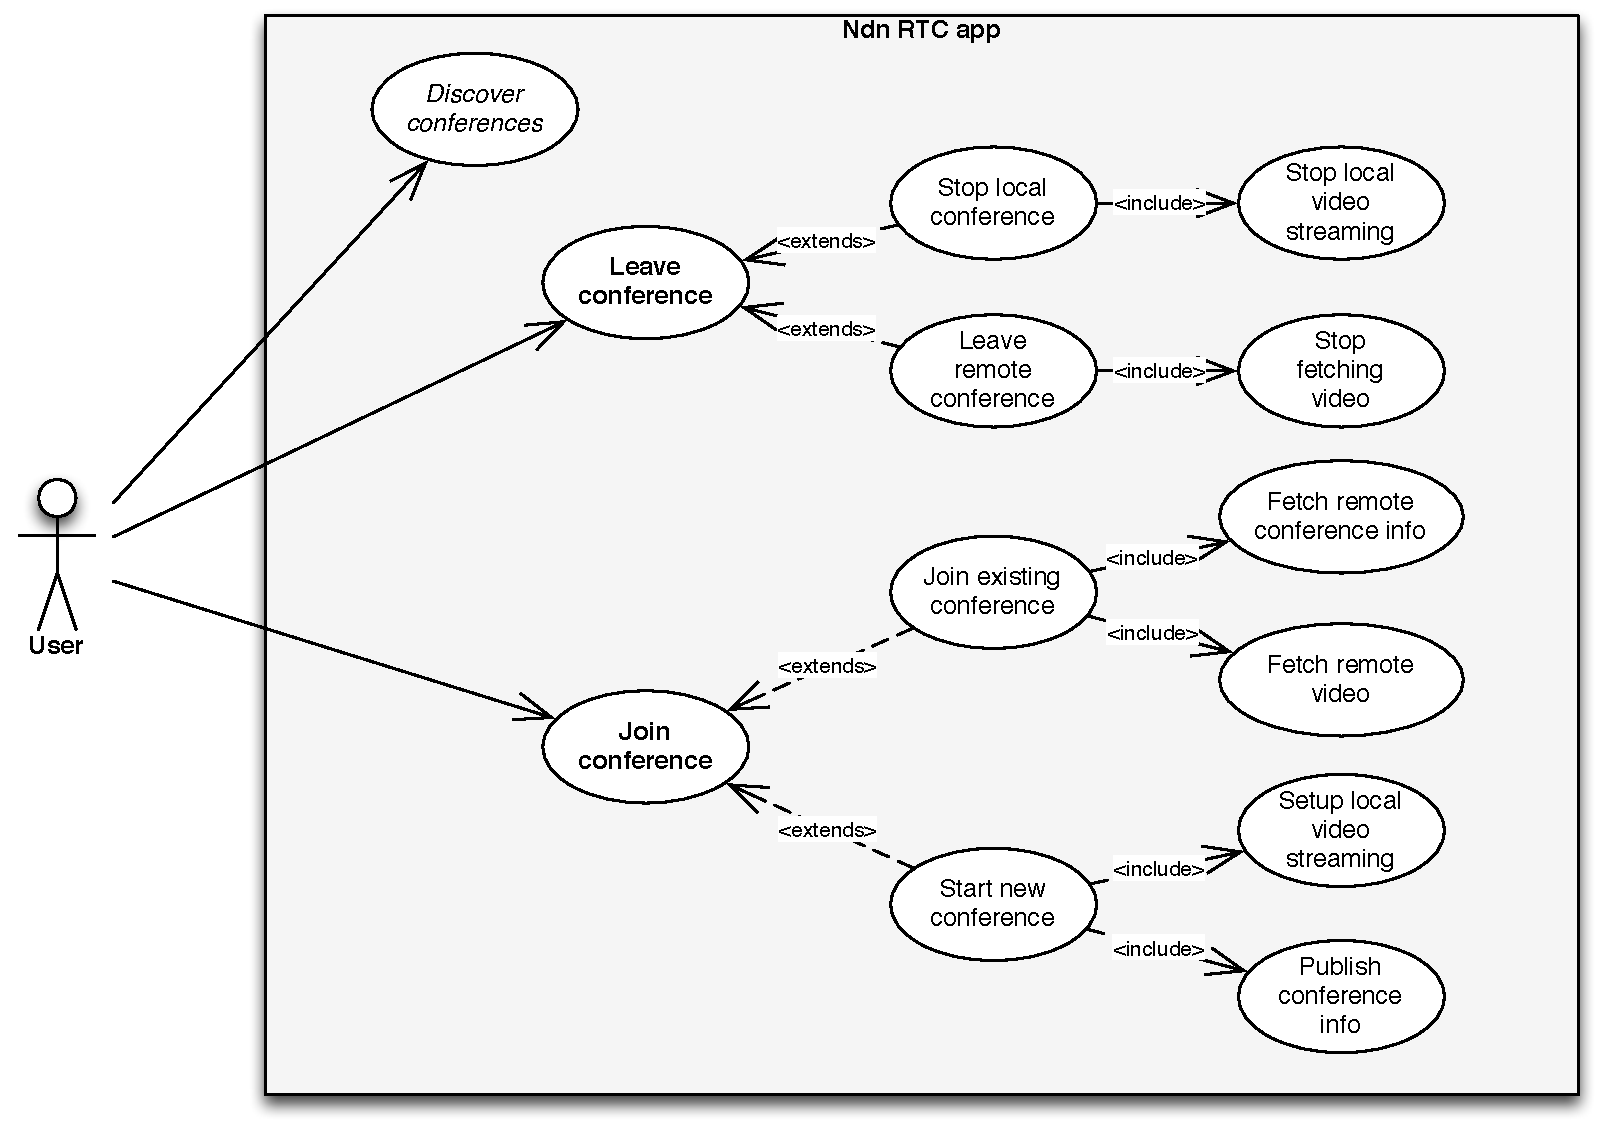
\includegraphics[width=\textwidth]{../res/graphics/addon-uc}
\caption{NDN-RTC Use-Cases}
\label{fig:uc}
\end{figure}

In order to satisfy easy-to-setup requirement, NDN-RTC was designed as a combination of Javascript and C++ modules which together operate inside Firefox browser. C++ module is responsible for real-time media communication and implemented as an add-on, while Javascript app provides all discovery functionality and UI (see Figure \ref{fig:arch}).

\begin{figure}[Ht!]
\centering
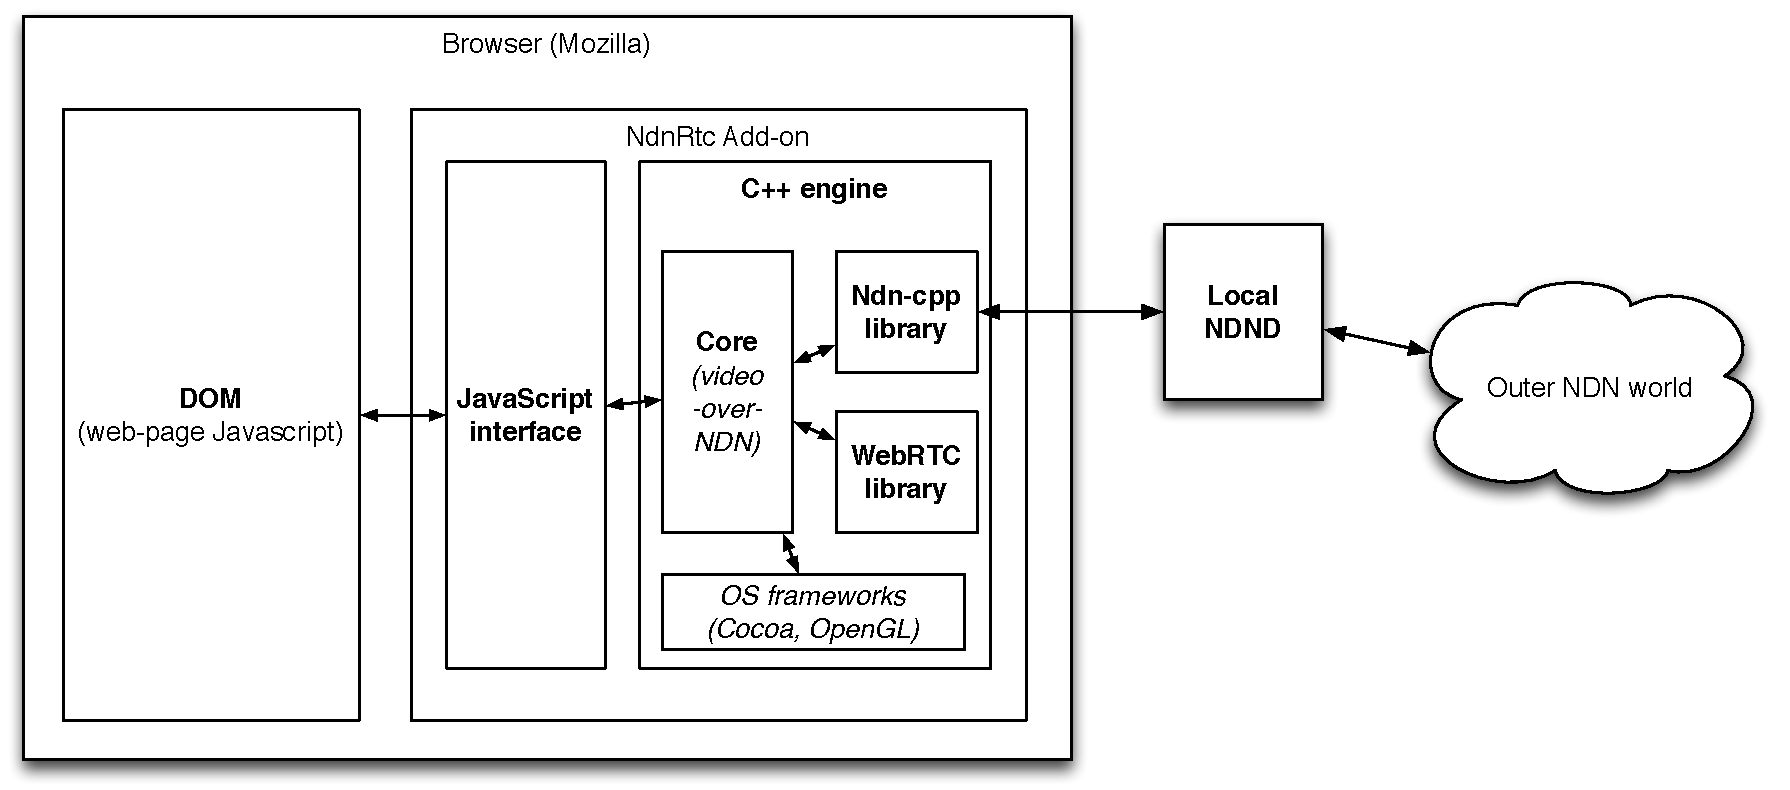
\includegraphics[width=\textwidth]{../res/graphics/addon-arch}
\caption{NDN-RTC architecture}
\label{fig:arch}
\end{figure} 

Two modules of NDN-RTC are: 
\begin{enumerate}
\item \textbf{NDN-RTC Add-on} \\
Add-on consists of several submodules, namely:
\begin{itemize}
\item \textbf{C++ engine}
\begin{itemize}
\item \textit{Core} - implements NDN-RTC protocol for enabling real-time media communication over NDN networks.
\item \textit{NDN-Cpp library} - provides interfaces for NDN-specific network interaction.
\item \textit{WebRTC library} - provides interfaces for media encoding/decoding, echo-cancellation, audio/video synchronisation, etc.
\end{itemize}
\item \textbf{Javascript interace} - provides Javascript API for web applications for accessing C++ engine functionality.  
\end{itemize}
\item \textbf{NDN-RTC Web App} \\
Provides general conference discovery between peers and UI.
\end{enumerate}

One should note that NDN-RTC Add-on is required to be installed in a browser for proper functioning of NDN-RTC Web App. In other words, without the add-on NDN-RTC Web App will not be able to provide RTC-over-NDN functions for its users, whereas add-on is solely independent module and the API it provides can be employed in third-party web apps. 

%The app borrows some ideas from previous work \cite{videoTR,ChronosTR}. It maintains synchronization of a digest tree in order to keep track of current chat participants in the same manner as ChronosChat \cite{ChronosTR}. Given that information, a new participant can start fetching media data objects from other peers (according to the media namespace presented on Figure \ref{media-ns}).
%
%\begin{figure}
%\centering
%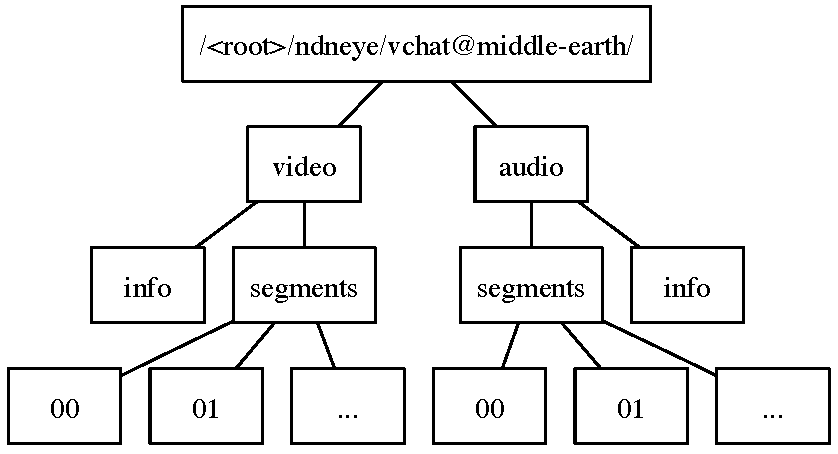
\includegraphics[width=0.8\textwidth]{../res/graphics/namespace-v01}
%\caption{NDN-WebRTC Media Namespace}
%\label{media-ns}
%\end{figure}
%
%The main goal of fetching media is to minimize the delay of receiving the latest frames. Having that in mind, we came up with the following design assumptions:
%
%\begin{itemize}
%\item Consumers are in full control of the speed of issuing media interests (i.e. interests in a segment namespace);
%\item Most recent media frames are delivered by pipelining media interests at an a priori higher rate than the producer delivers them (since the peer can obtain framerate information from the other peer by questioning the "info" namespace, it can determine the frequency of interest issuing);
%\item The presence of outstanding interests indicates retrieval of the most recent data;
%\item If the consumer has no outstanding interests, she increases the interest rate or, depending on the average rendering time, switches to a lower media quality. 
%\end{itemize} 
%
%Since no synchronization problems need to be solved in such a "consumer" approach, we hope that NDN-WebRTC can show better results in scalability for many-to-many scenarios.

\section{Protocol specification}
\subsection{NDN Namespaces}

Naming is an important aspect of any NDN application. There are three different namespaces used in NDN-RTC app: 
\begin{itemize}
\item \textbf{user namespace} - used for accessing individual user's media data and peer-to-peer session initiation (see Figure \ref{fig:ns});
\item \textbf{session namespace} - used for accessing conferences' info (both peer-to-peer and many-to-many) and encrypted ChronoChat room;
\item \textbf{discovery namespace} - used for discovery mechanisms (see Section \ref{sec:discovery} for details).
\end{itemize} 

\begin{figure}[Ht!]
\centering
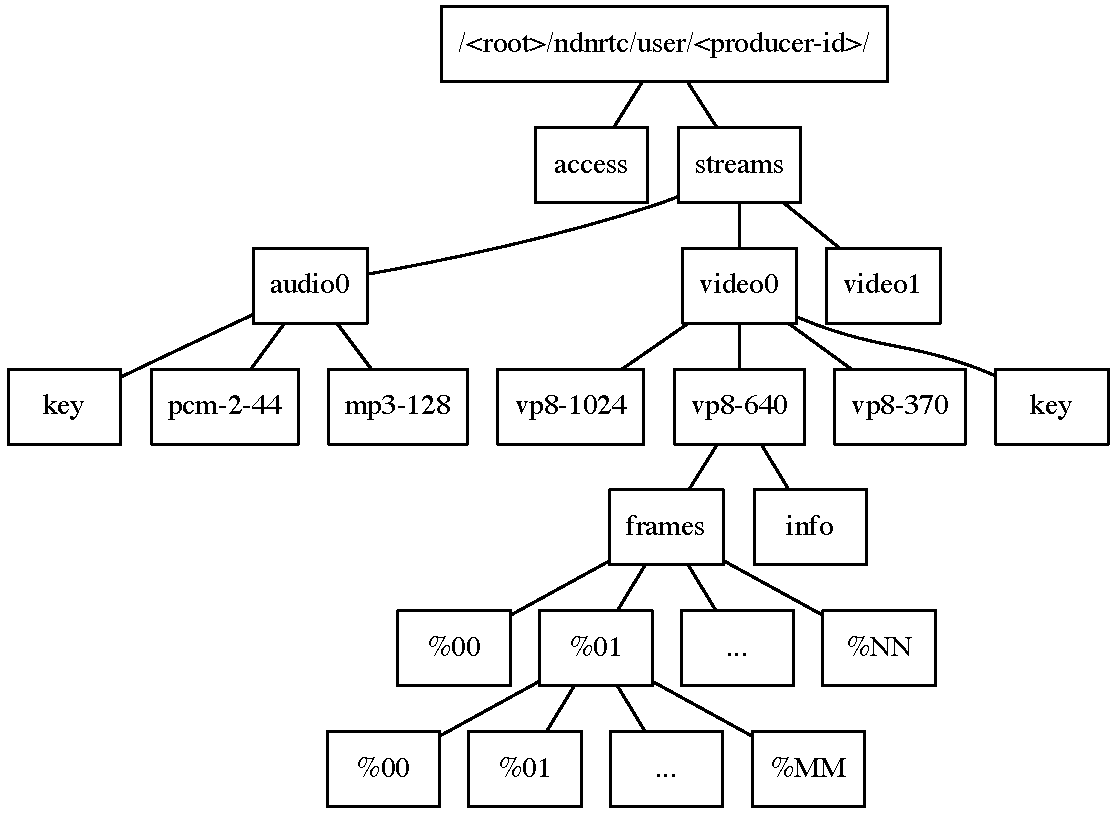
\includegraphics[width=0.9\textwidth]{../res/graphics/namespace}
\caption{NDN-RTC user namespace}
\label{fig:ns}
\end{figure}

Each user of NDN-RTC app is uniquely identified by a prefix URI which contains username (top level on the Figure \ref{fig:ns}). A user (further called a \textit{producer}) publishes her media streams (means audio or video streams) under \textit{streams} namespace as presented in Figure \ref{fig:ns}. Each stream is encoded with its own symmetric key (see Section \ref{security} for details). Producer can publish one particular stream in several copies with different encoding parameters (for instance, to allow consumers fetch media stream wich is the most appropriate for current network conditions). The information about streams' encoding parameters can be accessed by issuing interest in producer's \textit{info} namespace (\textbf{\textit{/$<$user prefix$>$/streams/video0/vp8-640/info}}) which will be satisfied by content object presented in Table \ref{tab:params}.

\begin{table}
\centering
\caption{Data object example for stream's "info" namespace}
\vspace{1em}
\small{
\begin{tabular}{|c|}
\hline
\textbf{/$<$user prefix$>$/streams/video0/vp-640/info}\\
\hline
StartTime: 1379894400 \\
\hline
Type: "video" \\
\hline
Codec: "vp8" \\
\hline
Framerate: 30 \\
\hline
Bitrate: 4000 \\
\hline
\textbf{Producer's Signature} \\
\hline
\end{tabular}}
\label{tab:params}
\end{table}

Any user who wants to fetch producer's media stream (further called a \textit{consumer}) needs to express interest with URI corresponding to a certain media stream (see Section \ref{sec:rtc} for more details on RTC). 

All type of communications inside NDN-RTC (whether it is peer-to-peer or many-to-many conference) are uniquely identified by \textit{sessions}. Each session has an initiator and participants. Session should have at least two participants to be initiated. Each session has a description (see Figure \ref{fig:conf-struct}), which contains such information as participant list, encryption key, conference name, description, etc. NDN-RTC sessions are placed under the session namespace:

\begin{center}
\textbf{\textit{/$<$root$>$/ndnrtc/session/$<$session-id$>$}}
\end{center}

This prefix is used as a ChronoChat URI. However, there are several modifications to the traditional ChronoChat protocol \cite{ChronoTR}. First, in addition to the existing ChronoChat namespace, a new \textit{info} node is added. By issuing interests in this namespace (\textbf{\textit{/$<$root$>$/ndnrtc/session/$<$session-id$>$/info}}) users can access conference announcement information. NDN-RTC adopts Audio Conference Tool approach \cite{act-sec} for secured conference announcements (see Section \ref{security} for details).

Moreover, several additional control message types were added to the existing ChronoChat messages. These messages are used for propagating service information among participants like added/removed media streams, changing encryption keys, etc. (see Table \ref{tab:msgs}). 

\begin{table}
\centering
\caption{NDN-RTC conference service messages}
\vspace{1em}
\small{
\begin{tabular}{|p{0.3\textwidth}|p{0.3\textwidth}|p{0.4\textwidth}|}
\hline
Type & Parameters & Description \\
\hline
\textit{StreamChanged} 
& \vspace{-1.8em} \begin{itemize} 
\item{media stream prefix}
\item{type of change: \textit{added, removed}}
\end{itemize} & Message is sent anytime user adds or removes a stream from an ongoing conference. \\ 
\hline
\textit{StreamKeyChange}
& \vspace{-1.8em} \begin{itemize} 
\item{media stream prefix}
\item{frame number}
\item{encryption key}
\end{itemize} & Message is sent when producer changes encryption key for a media stream. The new key should be used after the specified frame number. \\ 
\hline
\textit{ConferenceInfoUpdate}
& & Message is sent when conference initiator changes any conference description data. Other participants can fetch new version of conference data after receiving this message. \\ 
\hline
\end{tabular}}
\label{tab:msgs}
\end{table}

There is a third namespace used in NDN-RTC which allows users to discover current conferences and each other called discovery namespace. Next section \ref{sec:discovery} explains it in detail. 

\subsection{Discovery}
\label{sec:discovery}
In order to start a chat session (either video, audio or textual) between two peers, at least one peer need to know name prefix of the other one. Likewise, users need a mechanism for conferences discovery. NDN-RTC app provides these two types of discoveries: 
\begin{itemize}
\item \textbf{User discovery} - allows to see currently "active" or "visible" users of NDN-RTC.
\item \textbf{Conference discovery} - allows to see current ongoing conferences. 
\end{itemize}

Either type of discovery is essentially implemented in the same way using existing ChronoChat protocol with a restriction to allowed message types. Once a user started NDN-RTC app and would like to be visible for other users, she joins (sends a \textit{Join} message) to a global service chat room with the prefix: \textbf{\textit{/ndn/broadcast/ndnrtc/roster}}. It's a special chat room which does not allow any type of data messages except \textit{Join}, \textit{Leave} and \textit{Heartbeat}. In all other respects, it is treated as usual ChronoChat room with syncing, recovery, etc. and each user who joins this room (which basically in this context means "become visible to other users") is synced with chat room data automatically by the means of ChronoChat protocol. By providing name prefixes in \textit{Join} messages (either for a user or a conference, see Figure \ref{fig:tree}) users can easily fetch these prefixes and initiate new or join existing sessions. Users who'd like to stay visible should send \textit{Heartbeat} messages periodically. The same ideas of joining system roster chat room applies for conferences as well.

\begin{figure}[Ht!]
\centering
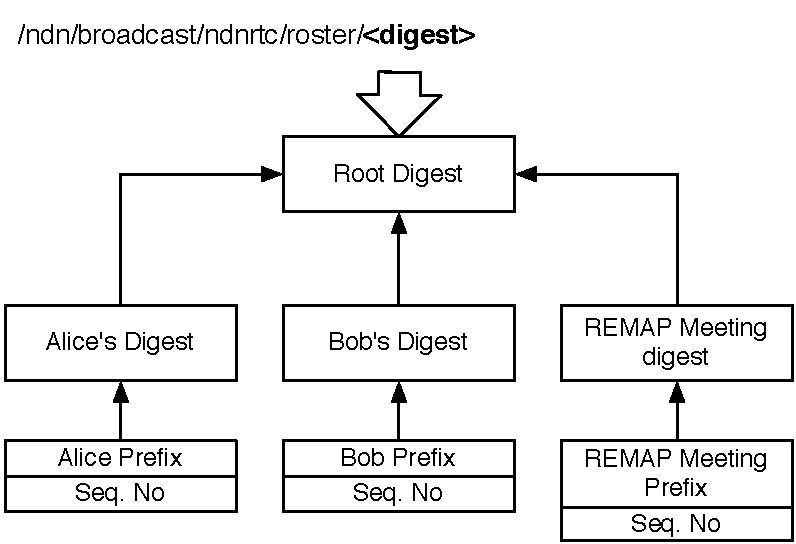
\includegraphics[width=0.7\textwidth]{../res/graphics/tree}
\caption{NDN-RTC discovery ChronoChat digest tree}
\label{fig:tree}
\end{figure}

\subsection{Real-time communication}
\label{sec:rtc}
\begin{enumerate}
\item Upon successful discovery of a video producer URI, the consumer issues an interest in the index namespace and gets data about the media stream's parameters ($FrameRate$ and codecs).
\item The consumer issues $Interest_{0}$ with the \textit{RigthMostChild=\textbf{true}} selector in the namespace for the frames like this: \textit{/root/mediadata} and waits until the first segment is received.
\item The consumer switches to \textbf{"Chase Mode"}
\end{enumerate}

\textbf{Chase Mode}
\begin{enumerate}
\item THe consumer extracts the frame number - $FN$ from the obtained $DataObject$ and pipelines interests at a rate of $2*FrameRate$ (twice the producer data rate) with \textit{RightMostChild=\textbf{true}} in the namespace for segments like this: \textit{/root/mediadata/FN/0}. i.e. the pipeline contains interests $Interest_{FN}$, $Interest_{FN+1}$, $Interest_{FN+2}$,...

\item The consumer watches two parameters: $DeliveryRate$ of frames, $RoundTripTime$ for interests:
\begin{itemize}
\item If $DeliveryRate$ is the same as $FrameRate$  and $RoundTripTime$ is not growing steadily, the consumer switches to \textbf{Fetch Mode} (see below)
\item If either $DeliveryRate$ and/or $FrameRate$ are growing, the consumer chooses a lower quality (by modifying the prefix) and re-enables \textbf{Chase Mode}
\end{itemize}
\end{enumerate}

\textbf{Fetch Mode}
\begin{enumerate}
\item The consumer extracts the latest frame number - $LFN$ and sets up a \textit{Frame interest} pipeline at a frequency of $2*FrameRate$:
\begin{center}
for a 24 fps video:
\begin{itemize}
\item \textbf{t = 0 sec} \\
Interest for \textit{/root/video/LFN/0}, timeout = 1.5 sec
\item \textbf{t = 1/48s} \\
Interest for \textit{/root/video/LFN+1/0}, timeout = 1.5 sec
\item \textbf{t = 2/48s} \\
Interest for \textit{/root/video/LFN+2/0}, timeout = 1.5 sec
\item ...
\end{itemize}
\end{center}

The number of segments per frame ($NumSegs$) is indicated using the \textit{FinalBlockID} field of each segment's DataObject. The consumer sets up a \textit{Segments interest} pipeline for each frame like this: 
\begin{center}
\begin{itemize}
\item Interest for \textit{/root/video/LFN/0}
\item Interest for \textit{/root/video/LFN/1}
\item Interest for \textit{/root/video/LFN/2}
\item ...
\item Interest for \textit{/root/video/LFN/$SegNum$}
\end{itemize}
\end{center}

\item The consumer periodically issues a \textbf{"probe"} interest with the last known frame number and \textit{RightMostChild=\textbf{true}} in order to detect a lag from the producer. If a considerable lag was detected, the consumer chooses stream parameters for a lower rate and switches to the \textbf{Chase Mode}

\item The consumer watches the value of $DeliveryRate$ and $RoundTripTime$ for the interests. If either of these values starts to grow, the consumer should choose stream parameters for a lower rate and switch to the \textbf{Chase Mode} in order to minimize the lag from the producer.

\end{enumerate}

\subsection{Security concerns}
\label{security}
In order to provide secure communication between users, two main security problems should be solved:
\begin{enumerate}
\item Data encryption and verification
\item User authenticity
\end{enumerate}

\paragraph{Encryption and verification.} 

As NDN-RTC app requires communications over untrusted network, transmitted data should be encrypted. Moreover, as there is a requirement of real-time communication, encryption should be efficient enough in order to minimize the delay. In this case, choosing fast symmetric encryption over a slower asymmetric encryption is more preferable. 
Once user started to publish media stream (either audio or video), a new encryption key is created and the data is published encrypted by this key.

Data verification is achieved by leveraging NDN embedded mechanisms for per-packet signing. Therefore, consumer can verify received packet by checking it's signature.

\paragraph{Authenticity.} 

NDN-RTC app should be perceived in a "producer-consumer" approach, i.e. there is a producer of media data somewhere on the network, and there is a consumer who'd like to get access to the producer's data. In this case, a producer should be the only authority who is in charge of giving access to his/her data.

As producer's data is encrypted using symmetric key, producer can control access to his data by sending this key only to trusted users. Any consumer who wants to get access for  media stream from a producer needs to retrieve an encryption key first by issuing interest in the \textit{key} namespace of a media stream by adding his name and a timestamp:

\begin{center}
\textbf{\textit{/$<$producer prefix$>$/streams/video0/key/$<$caller$>$/$<$timestamp$>$}}
\end{center}

Adding a current timestamp prevents network from responding with previously cached data. Encryption key is returned to the consumer in a data object encrypted by the consumer's public key. 

A producer can change encryption keys for media streams anytime and notify other conference participants using \textit{StreamKeyChange} service chat message (see Table \ref{tab:msgs}). Per-stream encryption keys and ability to change them on-the-go makes feasible complex conference scenaria in NDN-RTC app: for instance, if a user participates in several conferences simultaneously, she can provide only audio stream in one conference, audio+video in another and screen sharing video in third conference. With per-stream keys other participants can not fetch media streams wich are not announced for the current conference.

\paragraph{Session announcement.}
Secured session announcement approach was borrowed from Audio Conference Tool (see \cite{act-sec} for details). Upon creation of new session, initiator generates a pair of keys $K_e$ and $K_d$ and symmetric session key $K_s$. Asymmetric keys are used for secure publishing of session's information, while symmetric key is used by all the participants for chat data encryption. A sample structure of session announcement packet is presented on Figure \ref{fig:conf-struct}. 

We assume, that public keys of all the participants accessible through the network and can be easily verified. Announcement data contains hashes of each participants' public key so they can quickly check, whether they are among invitees or not. If the user is among conference participants, she can retrieve encryption key $K_d$ and decrypt conference information as well as session key $K_s$. Using session key $K_s$, user can join conference straight away (by sending encrypted \textit{Join} message to the chat). 

\begin{figure}[Ht!]
\centering
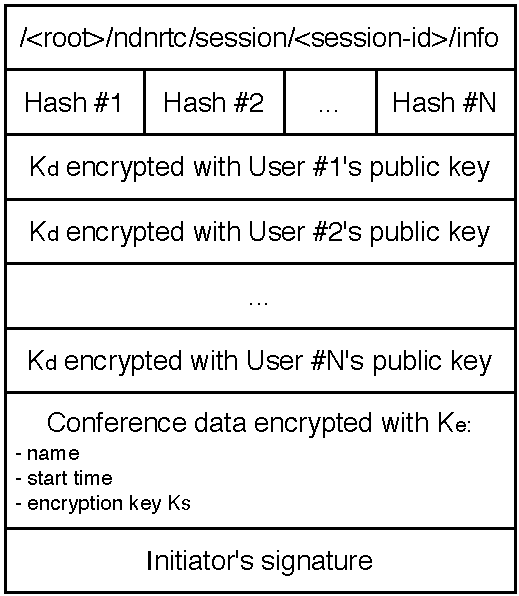
\includegraphics[width=0.5\textwidth]{../res/graphics/conf-struct}
\caption{Session announcement data}
\label{fig:conf-struct}
\end{figure}

\subsection{Session initiation}
\subsubsection{Peer-to-peer}
Initial interaction of two users is depicted by Figure \ref{fig:p2p}.

\begin{figure}[Ht!]
\centering
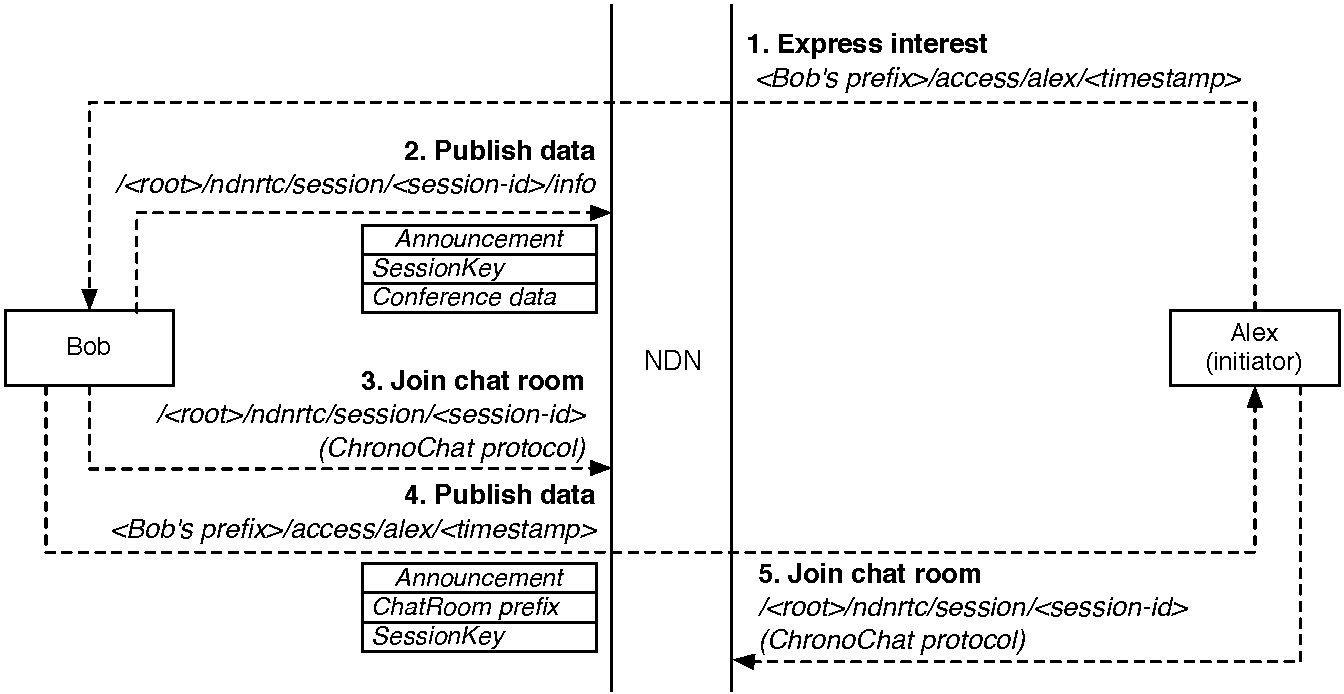
\includegraphics[width=\textwidth]{../res/graphics/p2p}
\caption{NDN-RTC peer-to-peer session initiation}
\label{fig:p2p}
\end{figure}

The user who would like to make a call issues an interest in an \textit{access} namespace of a callee's prefix by adding his name and current timestamp:

\begin{center}  \textbf{\textit{/$<$root$>$/ndnrtc/user/$<$callee$>$/access/$<$caller$>$/$<$timestamp$>$}}
\end{center}

Timestamp is needed in order to prevent network from answering with previously cached data. If calle answers the call, she performs three consecutive steps:
\begin{itemize}
\item initiates a new session by generating session id and announcement data and publishes them in session's \textit{info} namespace;
\item creates new chat room with prefix \textbf{\textit{/$<$root$>$/ndnrtc/sessions/$<$session-id$>$}}
 and joins it (using ChronoChat protocol);
 \item sends session announcement with chatroom prefix back to caller encrypted by the caller's public key.
\end{itemize}

Upon receiving a session announcement, the caller joins the chatroom and starts communication session by exchanging service or text messages. 

\subsubsection{Many-to-many}

In many-to-many scenario, unlike in peer-to-peer mode, session initiator does not interact with any of the participants directly and creates new session by publishing announcement data object in session's \textit{info} namespace. It is up to participants how they can discover the chatroom prefix (for instance, initiator may publish it in the discovery namespace or send it via e-mail). By obtaining chatroom prefix, participants are able to fetch session announcement data, extract encryption session key and join a conference. Many-to-many scenario is presented on Figure \ref{fig:m2m}

\begin{figure}[Ht!]
\centering
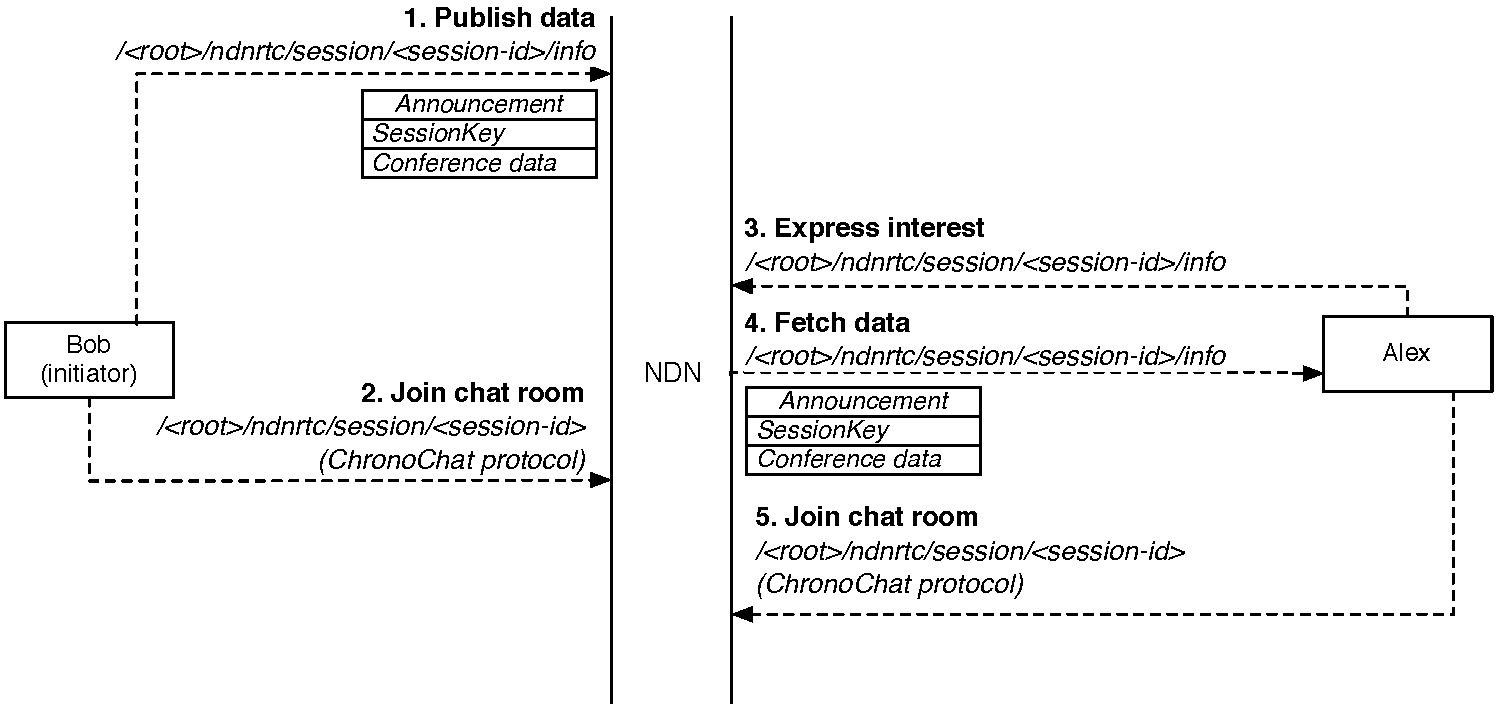
\includegraphics[width=\textwidth]{../res/graphics/m2m}
\caption{NDN-RTC many-to-many session initiation}
\label{fig:m2m}
\end{figure}

\section{App design}
\subsection{Overview}
\textit{TBD}
\subsection{C++ Firefox add-on}
\textit{TBD}
This sections describes the internal architectural approach for the C++ part of the add-on.

One can start learning how the add-on works by looking at the sequence diagrams of the main use-cases: Starting a conference (Figure \ref{fig:start}), Joining an existing conference (Figure \ref{fig:join}) and Leaving a conference (Figure \ref{fig:leave}).

\begin{figure}
\centering
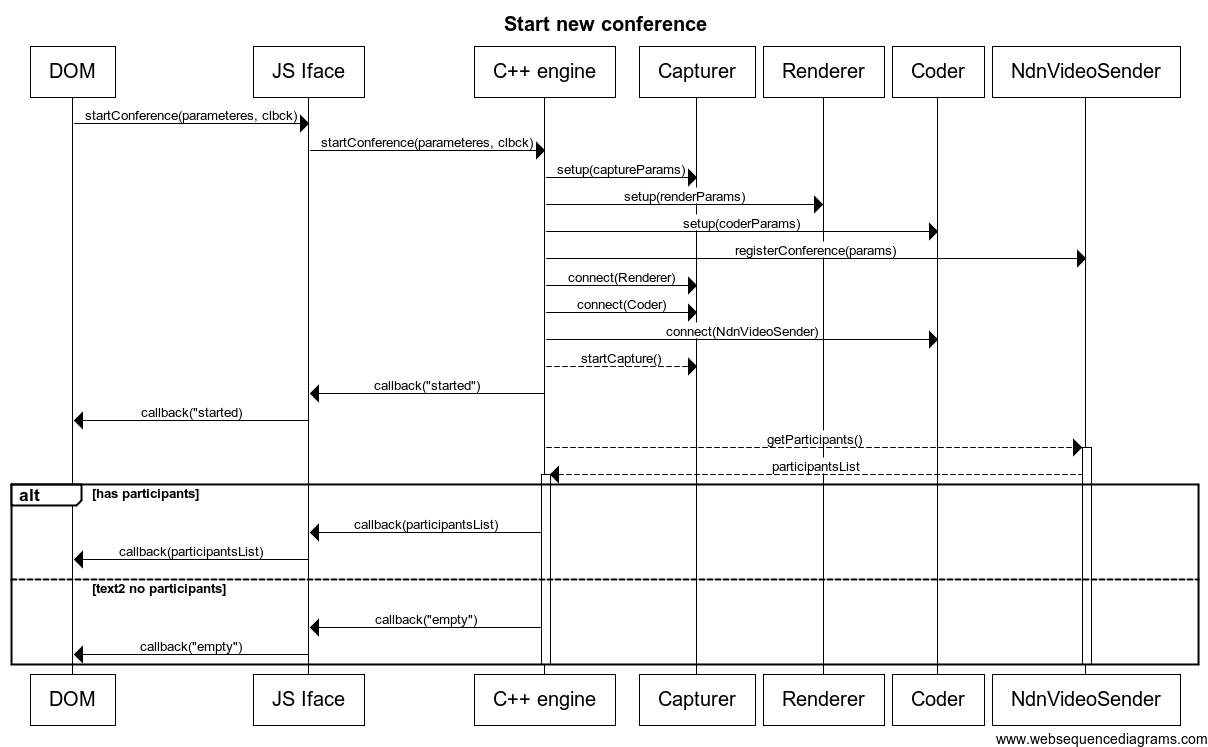
\includegraphics[width=\textwidth]{../res/graphics/start-seq}
\caption{Sequence diagram for starting a conference}
\label{fig:start}
\end{figure}

\begin{figure}
\centering
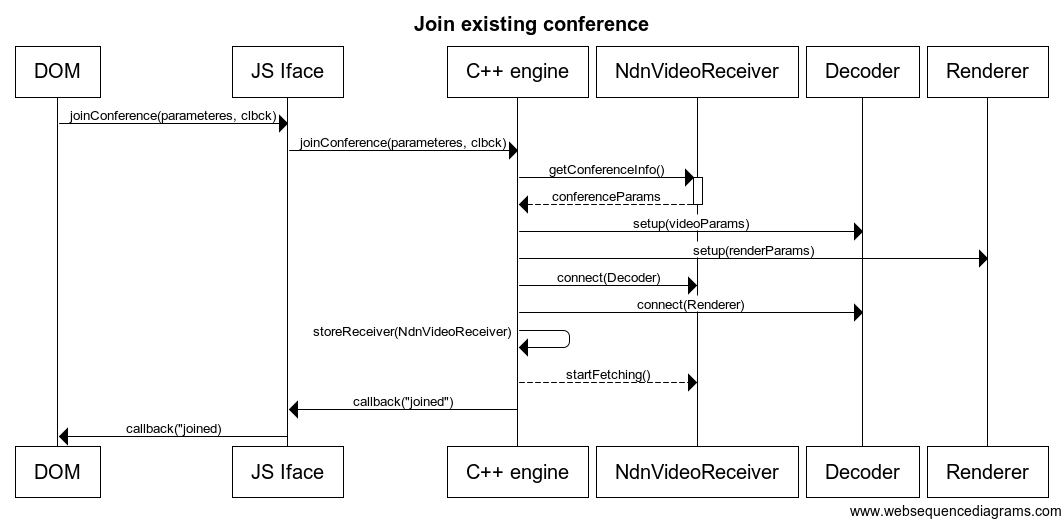
\includegraphics[width=\textwidth]{../res/graphics/join-seq}
\caption{Sequence diagram for joining an existing conference}
\label{fig:join}
\end{figure}

\begin{figure}
\centering
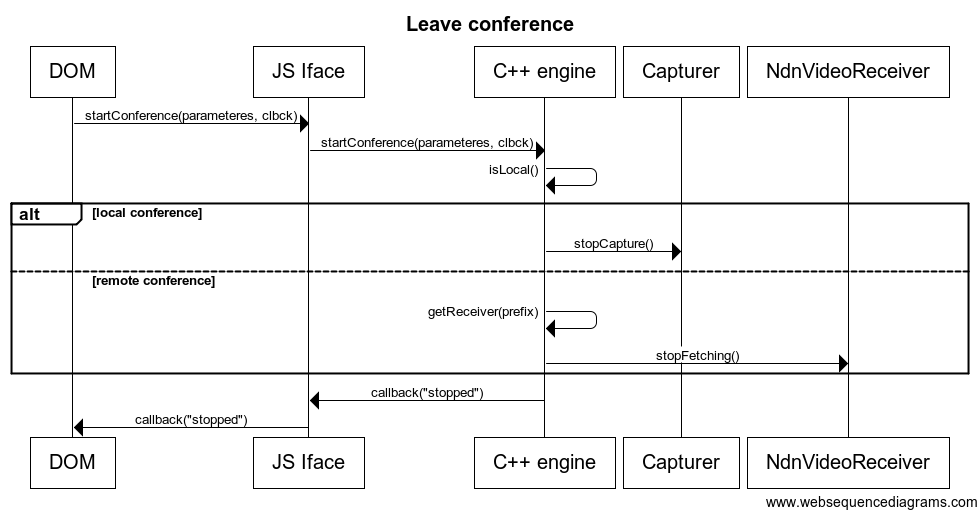
\includegraphics[width=\textwidth]{../res/graphics/leave-seq}
\caption{Sequence diagram for leaving a conference}
\label{fig:leave}
\end{figure}


\subsection{Javascript Web application}
\subsubsection{Overview}
\textit{TBD}
\subsubsection{UI design}
\textit{TBD}

\section{Next steps}
\begin{itemize}
\item Provide user authentication in video conferences
\item Implement secure media transfer
\item Scalable video encoding
\end{itemize}

\section{References} \cite{videoTR}, \cite{ChronosTR}
%************************************************
\bibliography{../res/bib/ndn-np}
\bibliographystyle{plain}



\end{document}